\newpage

\refstepcounter{section}
%Add Image
\vspace*{-40mm} %Make image have no top margin
\begin{tikzpicture}
\node[inner sep=0pt] (x) at (0,0)
    {\hspace{-87mm}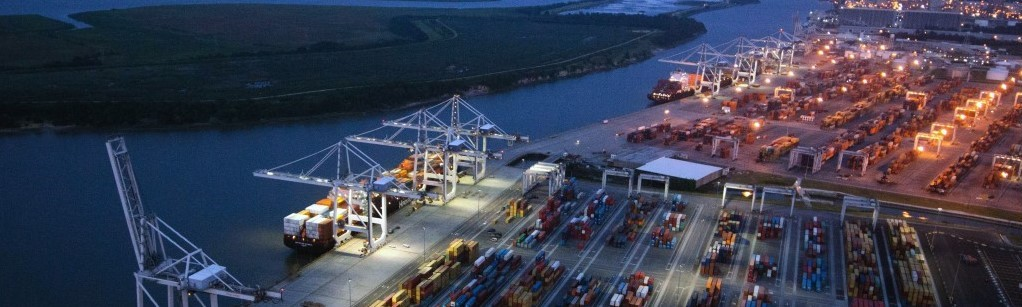
\includegraphics[width=\paperwidth]{sectionimage2.jpg}};
\node[text width=10in] (Z) at (0,-1) {\color{white}\headingfont\Large\bfseries\uppercase{\hspace{-0.7cm}\thesection\hspace{0.5cm}Stakeholder Requirements}};
\end{tikzpicture}
%Modify TOC
\addcontentsline{toc}{section}{\protect\numberline{\thesection}Stakeholder Requirements}
  \sectionmark{Stakeholder Requirements}
\vspace{-5mm}
  
%Content
\begin{multicols}{2}
\subsection*{Efficient Freight Transport}
    \begin{flushleft}
        \textbf{Stakeholders: }\textit{Transport Agencies, Port Users}
    \end{flushleft}
    \vspace{-3mm}
    Allow freight to be distributed within the North Island more efficiently.
\subsection*{Projected Economic Value}
    \begin{flushleft}
        \textbf{Stakeholders: }\textit{Central Government, External Councils, Auckland Council}
    \end{flushleft}
    \vspace{-3mm}
    Solution should provide short and long term economic opportunities to the chosen region, and allow the economic status of the country to grow and improve. 
\subsection*{Reduce Traffic Congestion in Auckland}
    \begin{flushleft}
        \textbf{Stakeholders: }\textit{Auckland Council/Residents, Transport Agencies, External Supporting Councils}
    \end{flushleft}
    \vspace{-3mm}
    Improving efficiency for all road and rail users, both public and private. 
\subsection*{Environmental Impacts and Resource Efficiency}
    \begin{flushleft}
        \textbf{Stakeholders: }\textit{Central Government, External Supporting Councils, Auckland Council/Residents, Transport Agencies, Investors}
    \end{flushleft}
    \vspace{-3mm}
    Sustainable and efficient use of natural resources in such a way that environmental impacts are reduced. Natural capital should be used as efficiently as possible.
\subsection*{Ensuring Safety}
    \begin{flushleft}
        \textbf{Stakeholders: }\textit{Central government, External Supporting Councils, Auckland Council, Transport Agencies, Investors}
    \end{flushleft}
    \vspace{-3mm}
    The devised solution must ensure paramount safety of involved parties at all stages of the project. 
\subsection*{Transparency}
    \begin{flushleft}
        \textbf{Stakeholders: }\textit{Central Government, External Supporting Councils, Auckland Council/Residents, Transport Agencies, Investors, Port users}
    \end{flushleft}
    \vspace{-3mm}
    Ensuring there is clear, effective and constant communication between all concerned parties, the government and the general public.
\subsection*{Economic Feasibility}
    \begin{flushleft}
        \textbf{Stakeholders: }\textit{Transport Agencies, Auckland Council, Central Government, External Supporting Councils, Investors}
    \end{flushleft}
    \vspace{-3mm}
    Ensure the project costs falls within the required budget and completion occurs within an appropriate time frame.
\subsection*{Public Approval}
    \begin{flushleft}
        \textbf{Stakeholders: }\textit{Auckland Council/Residents, External Supporting Councils, Investors}
    \end{flushleft}
    \vspace{-3mm}
    Taxpayers must not oppose how their money is being utilised during development.
    
\end{multicols}    


\clearpage